\section{Auswertung}

\noindent Für die Auswertung wurde zuerst der Dunkelstrom $I_{Dunkel}=\SI{5.6}{\nano\metre}$ gemessen. Dieser Wert wird im folgenden von den aufgenommenen Strömen abgezogen.\\
Zusätzlich wurde die Entfernung des Photoelements von dem Spalt zu $L=\SI{1.472}{\metre}$ gemessen.

\subsection{Auswertung des Einzelspaltes}

\noindent Für die Untersuchung der Beugungsmaxima wurde ein Spalt mit der Breite $b=\SI{0.15}{\milli\metre}$ genutzt.\\
Die aufgenommenen Messwerte sind in Tabelle \ref{tab:1} zu finden.\\ Über $\varphi=\frac{d}{L}$ lässt sich mit den Messwerten die Verschiebung des Photoelements in den benötigten Winkel umrechnen.

\begin{table}[ht]
    \centering
    \small
    \caption{Messdaten zur Messung des Photostroms beim Einzelspalt, in Abhängigkeit von der Verschiebung des Photoelements $d$ um die Mitte.}
    \label{tab:1}
    \begin{tabular}{S [table-format=2.2] S [table-format=3.1] | S [table-format=2.2] S [table-format=3.1]}
    \toprule
    {$d \mathbin{\scalebox{1.5} / } \si{\milli\metre}$} & $\text{Photostrom} \mathbin{\scalebox{1.5} / } \si{\nano\ampere}$ & {$d \mathbin{\scalebox{1.5} / } \si{\milli\metre}$} & $\text{Photostrom} \mathbin{\scalebox{1.5} / } \si{\nano\ampere}$\\
    \midrule
    -25    &   3  & 0.25 & 760   \\
    -23    &   1.5&   0.5  & 700   \\
    -21    &   1.5& 0.75 & 640   \\
    -19    &   7  & 1    & 560   \\
    -17    &   3.5&  1.25 & 500   \\
    -15    &   9  & 1.5  & 420   \\
    -13    &  12  &  1.75 & 360   \\
    -11    &   6  &  2    & 290   \\
    -10    &  17.5& 2.25 & 230   \\
     -9    &  32  & 2.5  & 180   \\
     -8    &  32  & 3    &  95   \\
     -7    &  16  &  3.5  &  40   \\
     -6    &  15.5&  4    &  15   \\
     -5    &  88  & 4.5  &  10   \\
     -4.5  & 170  & 5    &  19   \\
     -4    & 280  &   6    &  44   \\
     -3.5  & 400  & 7    &  47   \\
     -3    & 540  &  8    &  27   \\
     -2.5  & 670  &  9    &  10   \\
     -2.25 & 730  &   10    &   7.5 \\
     -2    & 780  & 11    &  15   \\
     -1.75 & 830  & 13    &  13.5 \\
     -1.5  & 860  &  15    &   3   \\
     -1.25 & 880  & 17    &   9   \\
     -1    & 900  & 19    &   4.5 \\
     -0.75 & 890  & 21    &   3   \\
     -0.5  & 880  &  23    &   5   \\
     -0.25 & 850  & 25    &   1   \\
      0    & 800  &       & \\
    \bottomrule
    \end{tabular}
  \end{table}


\noindent
Damit wird dann für eine Funktion der Form
\begin{equation}
    B(\varphi')^2 = A_0^2 \left\{ \frac{\lambda}{\pi b \text{ sin}(\varphi')} \right\}^2 \cdot \text{ sin}^2 
    \left\{\frac{\pi b \text{ sin}(\varphi')}{\lambda} \right\}
    \label{eqn:einzel}
\end{equation}
\noindent eine Ausgleichsrechnung durchgeführt. Des Weiteren gilt hier $\varphi'=\varphi-a$, da das Maximum der Messwerte nicht genau um $0$ zentriert ist und dies mit diesem Term kompensiert wird.\\
Die Parameter der Funktion berechnen sich dann zu
\begin{align*}
    A_0&=\SI{5.447(0012)}{\sqrt\ampere}\\
    a_1&=\SI{-0.648(0003)e-3}{\degree}\\
    b_1&=\SI{0.1734(00004)}{\milli\metre}\; \; .
\end{align*}
\noindent Zusammen mit den Messwerten finden sich diese Funktion grafisch dargestellt in Abbildung \ref{fig:plot1}.
\begin{figure}[H]
    \centering
    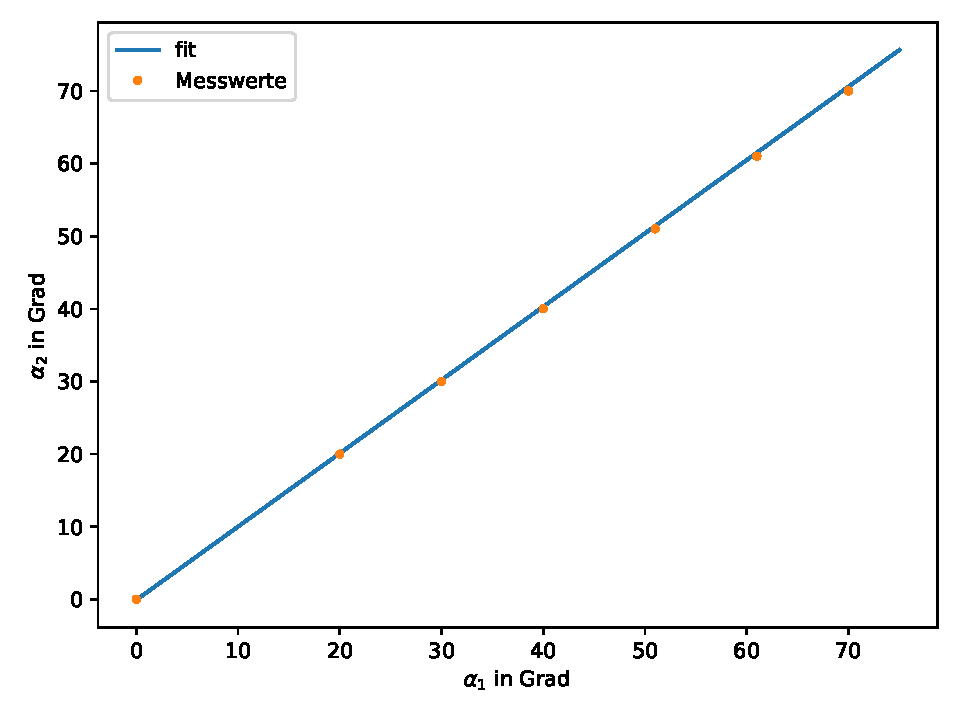
\includegraphics[width=0.55\textwidth]{build/plots/plot1.pdf}
    \caption{Die Messwerte der Intensitäten des Einzelspaltes inklusive der darauf bestimmten Ausgleichsfunktion.}
    \label{fig:plot1}
  \end{figure}



\newpage
  \subsection{Auswertung des Doppelspaltes}

  \noindent Für die Untersuchung des Doppelspaltes wurde ein Doppelspalt mit der Spaltentfernung $s =\SI{1}{\milli\metre}$ und der Spaltbreite $b={\SI{0.15}{\milli\metre}}$ genutzt.\\
  Hier wird die Funktion 
  \begin{equation}
    B(\varphi)^2 = A_0^2 \cdot \text{cos}^2 \left( \frac{\pi s \text{ sin}(\varphi')}{\lambda} \right) \cdot 
    \left\{ \frac{\lambda}{\pi b \text{ sin}(\varphi')} \right\}^2 \cdot \text{ sin}^2 \left\{ \frac{ \pi b \text{ sin}}{\lambda} \right\}^2 \; \;.
  \end{equation}
  Für die Ausgleichsrechnung genutzt. Dabei wurden wieder die Werte mit $\varphi=\frac{d}{L}$ umgerechnet und es gilt auch wieder $\varphi'=\varphi-a$.\\
  Die Parameter ergeben sich dann zu
  \begin{align*}
    A_0&=\SI{0.983(0054)e-3}{\sqrt\ampere}\\
    s&=\SI{0.9954(00171)}{\milli\metre}\\
    a_2&=\SI{0.588(0016)e-3}{\degree}\\
    b_2&=\SI{0.1740(00251)}{\milli\metre}\; \; .
  \end{align*}
  \noindent Zusammen mit den Messwerten finden sich diese Funktion grafisch dargestellt in Abbildung \ref{fig:plot2}.

  \begin{figure}[H]
    \centering
    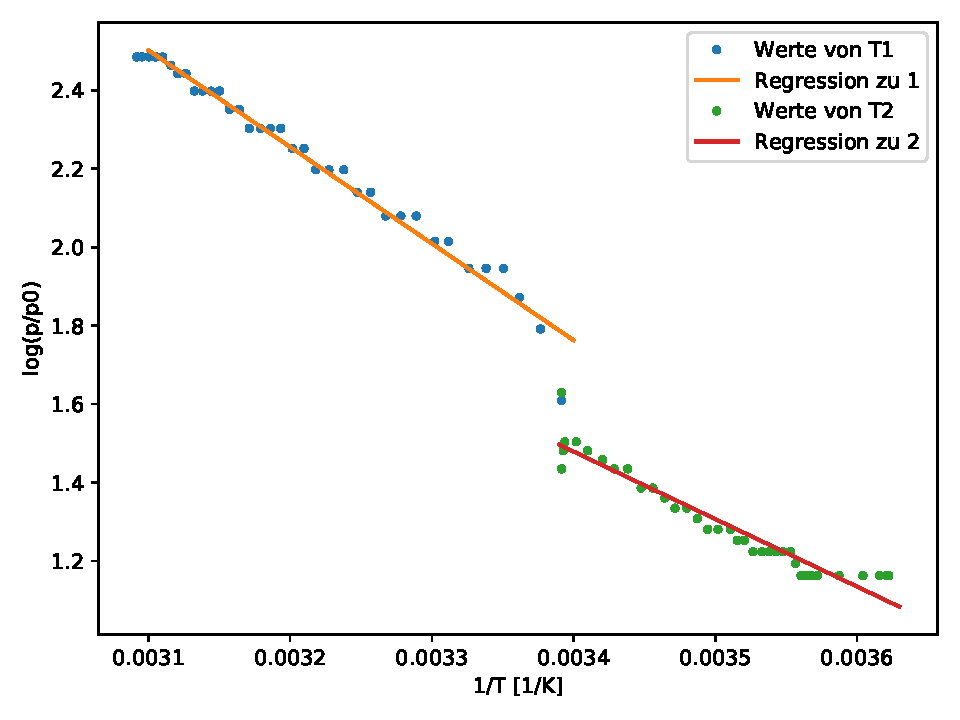
\includegraphics[width=0.6\textwidth]{build/plots/plot2.pdf}
    \caption{Die Messwerte der Intensitäten des Doppelspaltes inklusive der darauf bestimmten Ausgleichsfunktion.}
    \label{fig:plot2}
  \end{figure}
  \noindent Wenn nun beide Funktionen normiert und in eine Abbildung gesetzt werden sollte die Intensitätsfunktion des Einzelspaltes die Einhüllende der Doppelspaltfunktion sein.
  Dies ist in Abbildung \ref{fig:plot3} dargestellt. Es ist zu sehen, das dies gilt und die Funktionensehr genau aufeinander liegen.
  
  \begin{figure}[ht]
      \centering
      \includegraphics[width=0.6\textwidth]{build/plots/plot3.pdf}
      \caption{Die normierten Ausgleichsfunktion in einer Grafik aufgetragen.}
      \label{fig:plot3}
    \end{figure}

    \begin{table}[ht]
    \centering
    \small
    \caption{Messdaten zur Messung des Photostroms beim Doppelspalt, in Abhängigkeit von der Verschiebung des Photoelements $d$ um die Mitte.}
    \label{tab:tab2}
    \begin{tabular}{S [table-format=2.2] S [table-format=3.1] | S [table-format=2.2] S [table-format=3.1]}
        \toprule
        {$d \mathbin{\scalebox{1.5} / } \si{\milli\metre}$} & $\text{Photostrom} \mathbin{\scalebox{1.5} / } \si{\nano\ampere}$ & {$d \mathbin{\scalebox{1.5} / } \si{\milli\metre}$} & $\text{Photostrom} \mathbin{\scalebox{1.5} / } \si{\nano\ampere}$\\
        \midrule
        -25    &   0.25 &  0.25 & 620   \\
        -23    &   5    &  0.5  & 520   \\
        -21    &   2    &  0.75 & 500   \\
        -19    &   6    &  1    & 465   \\
        -17    &   7    &  1.25 & 360   \\
        -15    &   4.5  &  1.5  & 310   \\
        -13    &  13    &  1.75 & 280   \\
        -11    &   9.5  &  2    & 220   \\
        -10    &  12    &  2.25 & 160   \\
         -9    &  15    &  2.5  & 135   \\
         -8    &  17    &  3    &  70   \\
         -7    &  13.5  &  3.5  &  40   \\
         -6    &  14    &  4    &  10   \\
         -5    &  25    &  4.5  &  16   \\
         -4.5  & 135    &  5    &  22   \\
         -4    &  20    &  6    &  33   \\
         -3.5  & 310    &  7    &  27.5 \\
         -3    & 420    &  8    &  14   \\
         -2.5  & 520    &  9    &   5   \\
         -2.25 & 595    & 10    &   8.5 \\
         -2    & 610    & 11    &  12   \\
         -1.75 & 640    & 13    &   8   \\
         -1.5  & 705    & 15    &   7.5 \\
         -1.25 & 700    & 17    &   8   \\
         -1    & 700    & 19    &   2.5 \\
         -0.75 & 750    & 21    &   5   \\
         -0.5  & 700    & 23    &   8.5 \\
         -0.25 & 640    & 25    &   1.5 \\
          0    & 660    &       &       \\
        \bottomrule
    \end{tabular}
    \end{table}

